\section{Auswertung}

Anhand der genommenen Messgrößen kann der Radius der Öltröpfchen
und die Ladung dieser ermittelt werden. Die Messdaten sind in Tabelle \ref{tab: Messdaten}
aufgeführt.

\subsection{Bestimmung der Radien}

Der Radius eines vermessenen Öltröpfchens wird über Formel \eqref{eqn:Radius_Ohne} bestimmt.
Für die Bestimmung der Radien wird die Viskorität von Luft, die Fallgeschwindigkeit
und die Dichte des verwedeten Öles benötigt.
Aus den gemessenen Widerständen des Thermistors ist die Temperatur zu bestimmen. Diese wird für die Viskosität der Luft benötigt. Der Zusammenhang zwischen
Thermistorwiderstand und der Temperatur ist in \cite{anleitung01} in Form eine Tabell gegeben.
Anhand dieser Daten wurde eine Ausgleichsrechnung mit einem quadratischem Polynom
durchgeführt. Das Ergebnnis der Ausgleichsrechunng ist in Abb. \ref{fig:Temp}
einzusehen.

\begin{figure}
  \centering
  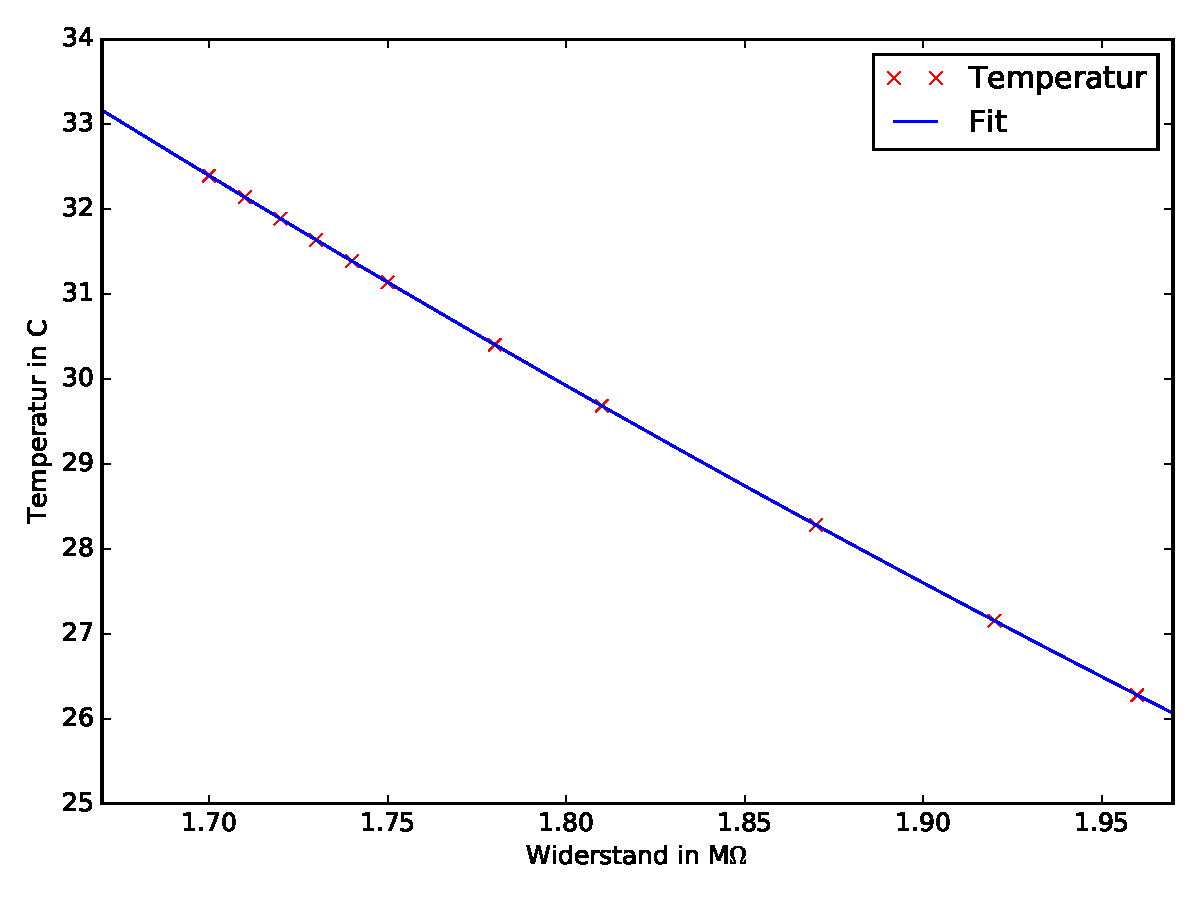
\includegraphics[width=\textwidth]{Pics/Temp.pdf}
  \caption{Gemessene Temperaturen.}
  \label{fig:Temp}
\end{figure}

Die Viskosität von Luft wurde mithilfe des Diagrammes aus \cite{anleitung01} bestimmt.
Dafür wurden zwei Punkte aus dem Diagramm abgelesen und die dazugehörige Geradengleichung ermittelt.
Die zu den gemessenen Temperaturen zugehörige Viskosität der Luft ist mittels der
Geradengleichung zu bestimmen.
Für die Dichte des verwendeten Öles wurde der Literaturwert
$\rho\ua{Oel} = \SI{886}{\kilogram\per\meter^3}$\cite{anleitung01} verwendet.
Die Fallzeit der Öltropfchen wurde über eine Strecke von $\SI{0,5}{\milli\meter}$
gemessen. Die Fallgeschwindigkeiten ergeben sich durch das teilen der Strecke durch
die gemessene Fallzeit.

Die berechneten Radien sind in Tab. \ref{tab: Messdaten} dargestellt. Alle Werte
sind als fehlerfrei angenommen worden, weshlab die Radien auch als fehlerfrei
betrachtet werden.

\subsection{Bestimmung der Ladung}

Die Ladung eines vermessenen Öltröpfchens wir über Formel \eqref{eqn:Ladung_korrigiert} ermittelt.
In dieser Formel ist der Korekturterm schon beinhaltet.
In die Berechnung der Ladung fließt die herrschende $E$-Feldstärke, der Radius des Öltröpfchens,
und der Druck mit ein. Die Konstante $B$ wurde in der Literatur \cite{anleitung01}
mit $\SI{6,17e-3}{\centi\meter}\su{Torr}$ angegeben. Als Druck wurde der
Atmosphärendruck mit $\SI{1.01325}{bar}$ verwendet.
Die $E$-Feldstärke ist durch die gemessene Spannung über den folgenden Zusammenhang
festgelegt.

\begin{equation}
  E = \frac{U}{d}
\end{equation}

Die Spannungen $U$ sind in Tabelle \ref{tab: Messdaten} einzusehen. Der Abstand
zwischen den Kondensatorplatten ist mit $\SI{7.6250 (51)}{\milli\meter}$ \cite{anleitung01}
angegeben.

Damit sind alle Größen zur Berechnung der Ladung eines Öltröpfchens gegeben. Die
berechneten Ladungen sind in Tabelle \ref{tab: Messdaten} einzusehen.

\begin{figure}
  \centering
  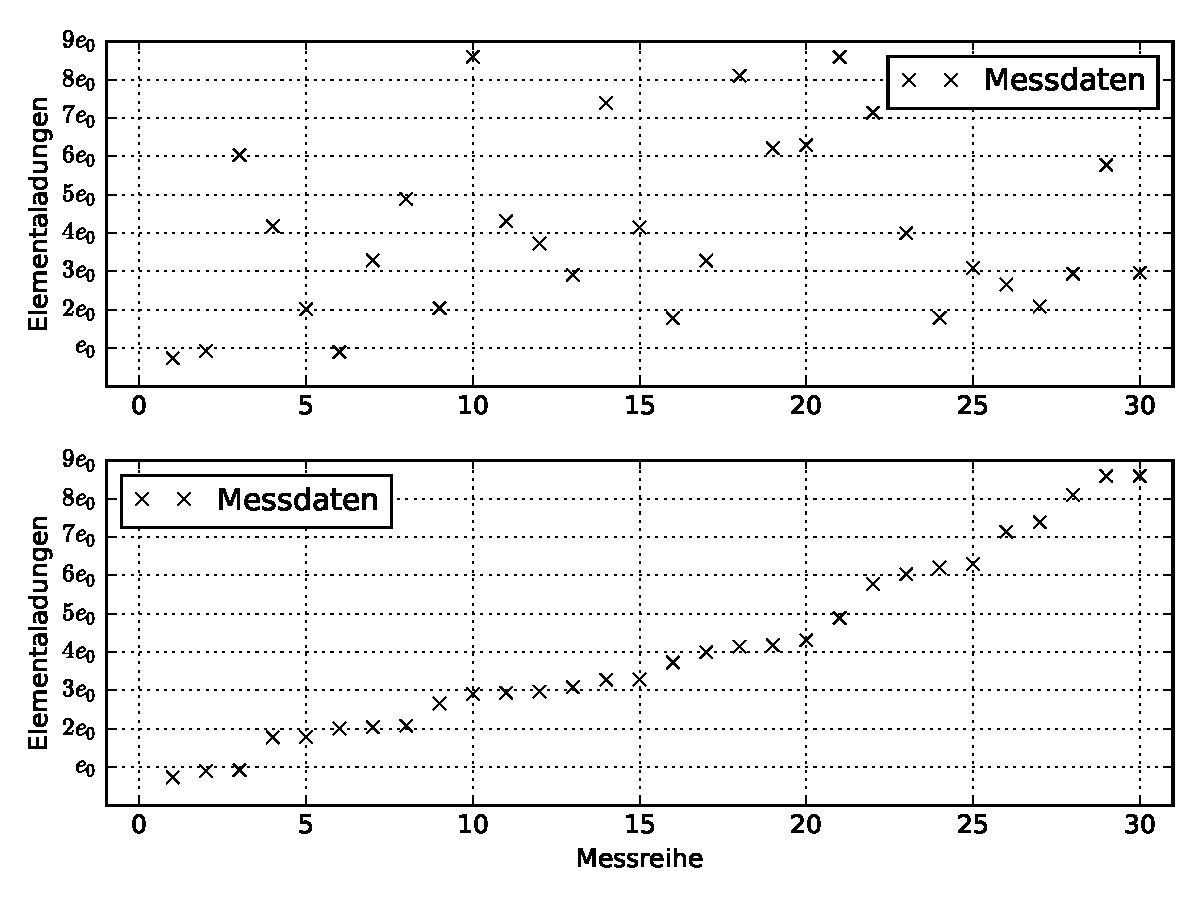
\includegraphics[width=\textwidth]{Pics/Ladungen_E_0.pdf}
  \caption{Ermittelte Ladungen. Das obere Diagramm zeigt die tatsächliche Messreihenfolge
  und das untere zeigt die bestimmten Ladungen der Größe nach sortiert.}
  \label{fig:Ladungen}
\end{figure}

Das Diagramm \ref{fig:Ladungen} zeigt die gemessenen Ladungen im Verhältnis zu der
Elementarladung. Die Elementarladung wurde aus dem \emph{SciPy}-Packet \emph{constants}
benutzt. Diese enspricht ungefähr einem Wert von $\SI{1,6022}{\coulomb}$.

Die Elementarladung entspricht der Ladung, die den größten gemeinsamen Teiler
aller gemessenen Ladungen bildet.
Damit diese bestimmt werden kann werden die Messdaten sortiert. Danach wurden für ähnliche Messdaten die
Mittelung aus diesen verwendet. Dies ist mit der Quantelung der Elementarladung zu begründen.
Ähnliche Messdaten müssen die selbe Elementarladung repräsentieren, da kein kontinuierliches
Spektrum an Messdaten zugelassen ist.
Der beste Kandidat für eine Elementarladung ist das Mininmum der im Folgendem dargestellten Menge.

\begin{equation}
  \su{min}\left\{\left|\su{rd}\left(\frac{Q}{Q\ua{Test}}\right) - \frac{Q}{Q\ua{Test}}\right|\right\}
\end{equation}

Als Testladungen wurde das Intervall $\left\{e_0 - 10^{-19}|e_0 + 10^{-19}\right\}$
verwendet. Das Intervall wurde so gewählt, da anzunehmen ist, dass die gemessene Elementarladung
in der Umgebung der tatsächlichen Elementarladung $e_0$ liegt.

Als gemessene Elementarladung ergibt sich der folgende Wert.

\begin{align}
  \label{eqn:Elementarladung}
  e\ua{gemessen} &= \SI{1,568e-19}{\coulomb} \\
  \label{eqn:abs_e_0}
  \left|\Delta_{e_0}\right| &= \SI{3,448e-21}{\coulomb}\\
  \label{eqn:rel_e_0}
  \delta_{e_0} &= \SI{0,022}{\coulomb}
\end{align}

$\Delta_{e_0}$ ist dabei der absolute und $\delta_{e_0}$ der relative Fehler.
Auf eine Fehlerrechnung wurde weitestgehend verzichtet, da auftretende Fehler lediglich aus
dem Abstand der Kondensatorplatten resultieren.

\subsection{Avogadro--Konstante}

Mit Hilfe der Faraday-Konstante $F$ und der Elementarladung lässt sich die
Avogadro-Konstante ermitteln. Die Größen hängen über die folgende Beziehung zusammen.

\begin{equation}
  \label{eqn:avogadro}
  N\ua{A} = \frac{F}{e_0}
\end{equation}

Es wurde der Wert der Faraday-Konstante aus dem \emph{SciPy}-Packet \emph{constants}
verwendet. Der Literaturwert der Avogadro-Konstante lautet $N\ua{A} = \SI{6,022e23}{\mol^-1}$.

Mit der berechneten Elementarladung ergibt sich die Avogadro-Konstante wie folgt.

\begin{align}
  \label{eqn:avogadro_gemessen}
  N\ua{A,gemessen} &= \SI{6,155e23}{\mol^{-1}} \\
  \label{eqn:abs_N_A}
  \left|\Delta_{N\ua{A}}\right| &= \SI{1.325e22}{\mol^{-1}}\\
  \label{eqn:rel_N_A}
  \delta_{N\ua{A}} &= \SI{0,022}{\mol^{-1}}
\end{align}


\section{Diskussion}

Möglich Fehlerquellen des Versuches sind in erster Linie Ablesefehler, da die
Zeitmessung mit einer Stoppuhr realisiert wurde. Zudem ist nicht auszuschließen,
dass die Fallbewegung der Öltropfchen vollständig horizontal und unbeeinflusst von
äußeren Einflüssen, wie Luftstöße war. Darüberhinaus ist die Viskositätsbestimmung der
Luft zu hinterfragen, da die bestimmte Geradengleichung aus abgelesenen Punkten
konstruiert wurde. Ablsesefehler wurden dabei vernachlässigt. Außerdem sind die Werte des
Thermistors in \cite{anleitung01} mit drei Nachkommastellen angegeben. Die
Widerstandsmessung ermöglichte jedoch nur Messungen auf bis zu zwei Nachkommastellen.


Das untere Diagramm aus Abb. \ref{fig:Ladungen} wurde der Übersichtlichkeit eingebunden.
Anhand dieses Diagrammes wurden die Mittel der Messdaten, wie in der Auswertung erwähnt,
bestimmt.
Der gequantelte Charakter der Ladung ist deutlich zu erkennen.

Die gemessene Elementarladung weicht um $\approx 2,2\%$ von dem Literaturwert ab.
Im Rahmen der Messgenauigkeit ist dieses Ergebnis erstaunlich präzise.

Die Avogadro-Konstante $N\ua{A}$ wurde bis auf $\approx 2,2\%$ Abweichung vom Literaturwert
wiedergefunden. Das Die Abweichung von $N\ua{A}$ und $e_0$ übereinstimmen liegt an dem
linear fortgepflanztem Fehler.
Dieses Ergebnis ist unter Betrachtung der Messmethode äußerst präzise.

Zusammenfassend ist zusagen, dass alle Messerwartungen vollkommen bestätigt wurden.

\section{Messdaten}

In diesem Kapitel sind die gemessenen und berechneten Größen tabellarisch
dargestellt.
In der Tabelle gelten die folgenden Bezeichnungen. $\Omega$ ist der gemessene
Widerstand des Thermistors, $t_0$ ist
die Zeit die ein Öltröpfchen ohne Feld für 0,5 mm benötigt, $\su{U}\ua{g}$
ist die Gleichgewichtsspannung, $r$ der bestimmte Radius des Öltröpfchens und
$q$ die berechnete Ladung dieses Öltröpfchens.

\begin{table}
\centering
\caption{Messdaten von V503.}
\label{tab: Messdaten}
\begin{tabular}{S S S S S S }
\toprule
{$\Omega$ in $\si{\mega\ohm}$} & {$t_0$ in $\si{\second}$} & {$\su{U}\ua{g}$ in $\si{\volt}$} & {$r$ in $\si{\nano\meter}$} & {$q$ in $10^{-20}\si{\coulomb}$} & {$\Delta_q$}  \\
\midrule
 1.96  & 17.78  & 269  & 520.69  & 11.72  & 0.01\\
1.92  & 29.26  & 96  & 406.42  & 14.77  & 0.01\\
1.87  & 35.03  & 11  & 372.06  & 96.64  & 0.06\\
1.81  & 15.76  & 58  & 555.83  & 66.97  & 0.04\\
1.78  & 34.00  & 35  & 378.83  & 32.21  & 0.02\\
1.71  & 23.20  & 147  & 459.76  & 14.38  & 0.01\\
1.75  & 15.41  & 77  & 563.31  & 52.64  & 0.04\\
1.75  & 6.83  & 187  & 846.13  & 78.35  & 0.05\\
1.75  & 11.40  & 200  & 654.93  & 32.71  & 0.02\\
1.75  & 6.61  & 112  & 860.09  & 137.70  & 0.09\\
1.74  & 9.93  & 118  & 701.98  & 69.04  & 0.05\\
1.74  & 18.00  & 53  & 521.39  & 59.74  & 0.04\\
1.73  & 19.26  & 61  & 504.23  & 46.62  & 0.03\\
1.73  & 13.78  & 41  & 596.12  & 118.39  & 0.08\\
1.73  & 9.40  & 134  & 721.77  & 66.36  & 0.04\\
1.72  & 20.30  & 92  & 491.33  & 28.44  & 0.02\\
1.73  & 11.56  & 122  & 650.85  & 52.58  & 0.04\\
1.72  & 6.84  & 113  & 846.43  & 129.81  & 0.09\\
1.72  & 13.58  & 50  & 600.71  & 99.48  & 0.07\\
1.72  & 15.49  & 40  & 562.46  & 100.85  & 0.07\\
1.71  & 8.49  & 76  & 760.02  & 137.67  & 0.09\\
1.71  & 9.55  & 76  & 716.60  & 114.39  & 0.08\\
1.71  & 8.13  & 175  & 776.66  & 64.00  & 0.04\\
1.71  & 15.55  & 140  & 561.58  & 28.67  & 0.02\\
1.71  & 9.03  & 192  & 736.94  & 49.45  & 0.03\\
1.70  & 12.13  & 140  & 636.07  & 42.60  & 0.03\\
1.70  & 16.18  & 113  & 550.74  & 33.38  & 0.02\\
1.71  & 12.67  & 118  & 622.14  & 47.12  & 0.03\\
1.70  & 6.95  & 155  & 840.32  & 92.51  & 0.06\\
1.70  & 14.95  & 90  & 572.95  & 47.54  & 0.03\\
\bottomrule
\end{tabular}
\end{table}

